\chapter{Synteza dźwięku - modulacja częstotliwości}\label{chapter_fm}
Modulacja częstotliwości jest powszechnie kojarzona z radiem analogowym. W tym zastosowaniu, zmiany częstotliwości fali nośnej są wykorzystane do przenoszenia sygnału audio do odbiorcy. W przypadku syntezy dźwięku, modulowane są dowolne sygnały okresowe. Nie niosą one żadnej informacji, a dewiacje (zmiany) częstotliwości chwilowej wprowadza się w celu uzyskania efektów dźwiękowych.
\section{Zasada działania modulacji częstotliwości}
Omawiana metoda polega na zmienianiu częstotliwości chwilowej przebiegu okresowego. Sygnał, którego częstotliwość podlega tym zmianom, nazywany jest sygnałem modulowanym lub nośnym. Zmiany wprowadzane w częstotliwości sygnału modulowanego, polegają na niewielkich zmianach jego częstotliwości własnej. Mogą one być dokonywane za pomocą innego sygnału, który nazywany jest sygnałem modulującym. 
\subsection{Modulacja FM w dziedzinie czasu}
Przykładem sygnału modulującego może być sinusoida. Przebieg zmodulowany częstotliwościowo, z pominięciem fazy sygnału modulującego \cite{oland}, opisuje wyrażenie:
\begin{equation} \label{equ:fm_wzor1}
S(t)= \text{sin}(2 \pi f_c t + \beta \text{sin}(2 \pi f_m t))
\end{equation}
\begin{tabular}{ l l l l}
	gdzie: & $t$ &  - & czas w sekundach, \\
	&	$f_c$ & - &  częstotliwość sygnału nośnego,\\
	&	$f_m$ & - &  częstotliwość sygnału modulującego,\\
	&	$\beta$ & - & amplituda sygnału modulującego.\\
\end{tabular} \\ \\
Na rysunku \ref{rys:fm_wykres1} zobrazowano modulację przeprowadzoną według (\ref{equ:fm_wzor1}) z parametrami: $\beta = 15, f_c = 1200, f_m = 55$.
\begin{figure}[H]
	\centering
	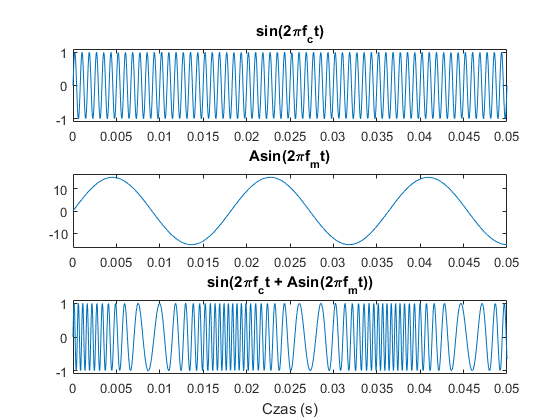
\includegraphics[width=12cm]{grafiki/fm_wykres1}
	\captionsetup{justification=centering}
	\caption{Prosty przykład sygnału zmodulowanego.}
	\label{rys:fm_wykres1}
\end{figure}
Na rysunku \ref{rys:fm_arg} przedstawiono przebiegi argumentów funkcji sinus z (\ref{equ:fm_wzor1}) dla pierwszych 50 milisekund sygnału.
\begin{figure}[H]
	\centering
	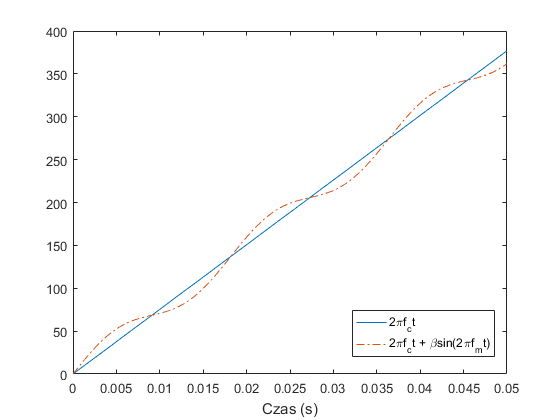
\includegraphics[width=10cm]{grafiki/fm_arg}
	\captionsetup{justification=centering}
	\caption{Przebiegi czasowe argumentu funkcji sinus przed i po modulacji FM.}
	\label{rys:fm_arg}
\end{figure}
Linią ciągłą narysowano przebieg argumentu sygnału nośnego przed modulacją. Natomiast linia przerywana obrazuje przebieg argumentu sygnału po modulacji częstotliwości.
\subsection{Modulacja FM w dziedzinie częstotliwości}
Wartość $\beta$ jest także określana mianem indeksu modulacji \cite{chowning}. Widmo sygnału poddanego modulacji częstotliwości składa się z prążka środkowego na częstotliwości nośnej oraz prążków bocznych. Prążki boczne są rozmieszczone symetrycznie względem częstotliwości nośnej i leżą na częstotliwościach $f_c \pm kf_m$, gdzie $k$ jest liczbą całkowitą. Moduł widma sygnału z powyższego przykładu przestawiony został na rysunku \ref{rys:fm_widmo}. Sygnał poddany transformacji Fouriera miał długość 96000 próbek przy $F_s = 96000$, zatem indeks częstotliwości uzyskanego widma jest równoważny częstotliwości rzeczywistej wyrażonej w Hz. Ze względu na sposób indeksowania w środowisku Matlab, zaczynający się od liczby 1 (a nie od 0), w celu uzyskania wartości częstotliwości należy odjąć jedynkę od indeksu.

\begin{figure}[H]
	\centering
	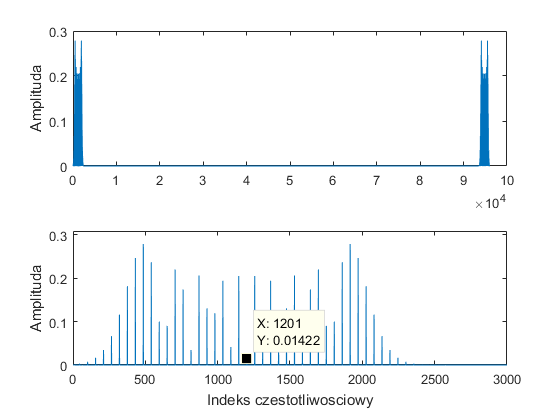
\includegraphics[width=10cm]{grafiki/fm_widmo}
	\captionsetup{justification=centering}
	\caption{Moduł widma sygnału zmodulowanego (wartość indeksu 1201 należy pomniejszyć o 1 ze względu na sposób indeksowania w środowisku Matlab).}
	\label{rys:fm_widmo}
\end{figure}
Wraz ze wzrostem wartości $\beta$, wzrasta liczba znaczących prążków bocznych oraz poszerza się pasmo częstotliwościowe sygnału zmodulowanego.
Wartości poszczególnych prążków odpowiadają wartościom funkcji Bessela typu pierwszego $J_n(x)$, gdzie $n$ jest rzędem. Wykresy tych funkcji dla trzech pierwszych rzędów przedstawione są na rysunku \ref{rys:fm_bessel}.
\begin{figure}[H]
	\centering
	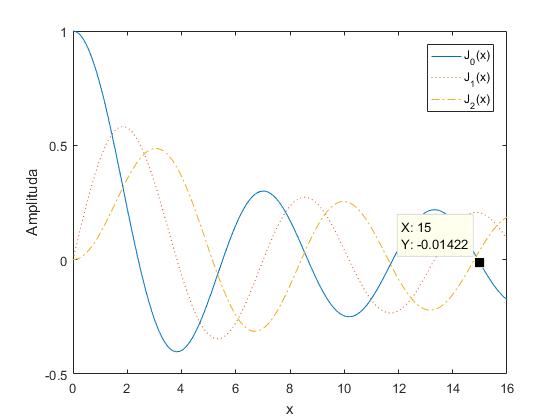
\includegraphics[width=10cm]{grafiki/fm_bessel}
	\captionsetup{justification=centering}
	\caption{Funkcje Bessela typu pierwszego.}
	\label{rys:fm_bessel}
\end{figure}

Moduł funkcji Bessela rzędu 0 w punkcie $\beta$ jest równy modułowi prążka na częstotliwości $f_c$. Moduł pierwszych prążków bocznych, tj. na częstotliwościach $f_c \pm f_m$ jest równy funkcji Bessela rzędu 1 w punkcie $\beta$. Postępując analogicznie można wyznaczyć moduły wszystkich znaczących prążków.

\subsection{Rozbudowana modulacja FM}
Zastosowanie modulacji FM w syntezie dźwięku ma doprowadzić do uzyskania efektów dźwiękowych. Zatem nic nie stoi na przeszkodzie, aby tę modulację rozbudowywać wedle własnego uznania. Można na przykład poddać modulacji przebieg modulujący. Niech sygnał modulujący (SM1) będzie modulowany przez SM2 (sygnał modulujący 2). Na rysunku \ref{rys:fm_modmod} przedstawiono wykresy sygnału nośnego, SM1, SM2 oraz sygnału końcowego, który jest opisany przez wzór:
\begin{equation} \label{equ:fm_modmod}
S(t)= \text{sin}(2 \pi f_c t + \beta \text{sin}(2 \pi f_m t + \gamma \text{sin}(2 \pi f_{m2} t)))
\end{equation}
\begin{tabular}{ l l l l}
	gdzie: & $t$ &  - & czas w sekundach, \\
	&	$f_c$ & - &  częstotliwość sygnału nośnego,\\
	&	$f_m$ & - &  częstotliwość SM1,\\
	&	$f_{m2}$ & - &  częstotliwość SM2,\\
	&	$\beta$ & - & amplituda SM1,\\
	&	$\gamma$ & - & amplituda SM2.\\
\end{tabular} \\ \\

\begin{figure}[H]
	\centering
	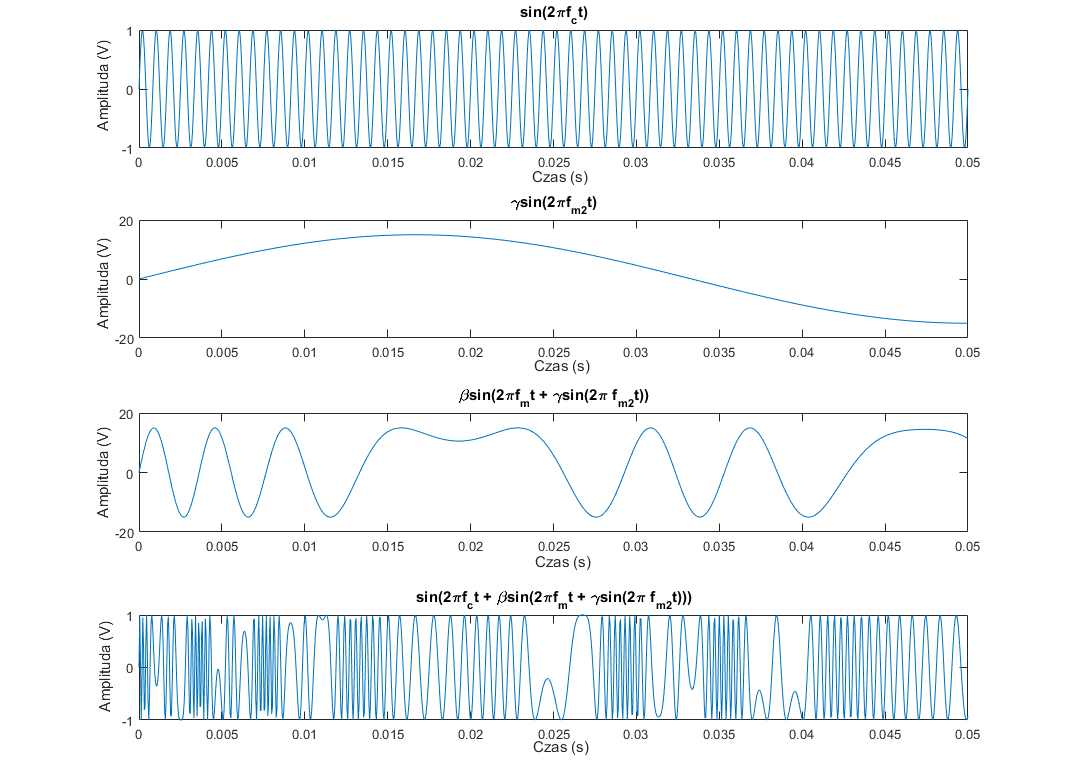
\includegraphics[width=14cm]{grafiki/fm_modmod}
	\captionsetup{justification=centering}
	\caption{Zagnieżdżona modulacja FM.}
	\label{rys:fm_modmod}
\end{figure}
Na rysunku \ref{rys:fm_arg2} przedstawiono przebiegi argumentów funkcji sinus z (\ref{equ:fm_modmod}) dla pierwszych 50 milisekund sygnału.
\begin{figure}[H]
	\centering
	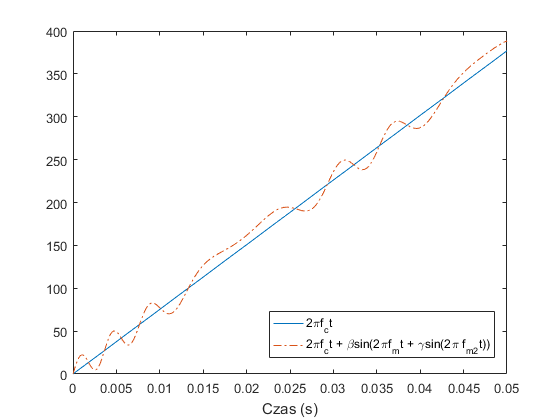
\includegraphics[width=10cm]{grafiki/fm_arg2}
	\captionsetup{justification=centering}
	\caption{Przebiegi czasowe argumentu funkcji sinus przed i po zagnieżdżonej modulacji FM.}
	\label{rys:fm_arg2}
\end{figure}
Linią ciągłą narysowano przebieg argumentu sygnału nośnego przed modulacją. Natomiast linia przerywana obrazuje przebieg argumentu sygnału po zagnieżdżonej modulacji częstotliwości. Na drodze eksperymentów można uzyskiwać w ten sposób naprawdę ciekawe brzmienia.
\subsection{Projektowanie brzmień}
W literaturze można znaleźć parametry syntezy FM, które pozwalają uzyskać brzmienie zbliżone do dźwięków naturalnych. W \cite{chowning} odnaleźć można na przykład parametry, za pomocą których można uzyskać brzmienie dzwonu. Parametry te wyglądają następująco:

\begin{table}[h!]
\centering
	\begin{tabular}{ |c| c| }
	\hline
	Parametr & Wartość \\
	\hline
	$f_c$ & 200 Hz \\
	\hline
	$f_m$ & 280 Hz\\
	\hline
	$\beta$ & 10\\
	\hline
	
	\end{tabular}
\captionsetup{justification=centering}
\label{tab:fm_bell}
\caption{Parametry brzmienia dzwona.}
\end{table}
Jednak dźwięk samego zmodulowanego przebiegu nie ma charakteru brzmienia dzwonu. Ważnym jest zastosowanie odpowiedniej obwiedni amplitudy uzyskanego przbiegu. W tym przypadku dobry wynik daje zastosowanie funkcji zanikającej ekspotencjalnie. Odpowiednim przykładem jest wyrażenie:
\begin{equation} \label{equ:fm_belladsr}
A(t) = e^{-t}.
\end{equation}
Przebieg obwiedni opisanej za pomocą (\ref{equ:fm_belladsr}) pokazano na rysunku \ref{rys:fm_belladsr}.
\begin{figure}[H]
	\centering
	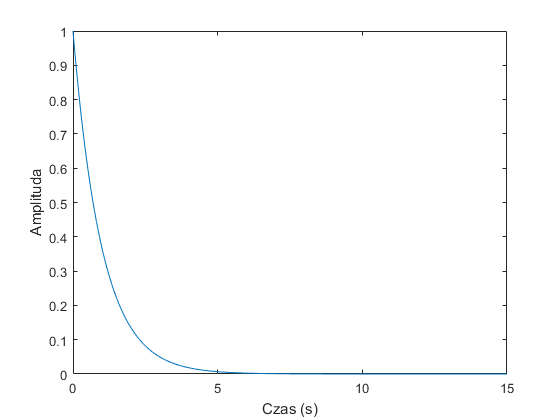
\includegraphics[width=10cm]{grafiki/fm_belladsr}
	\captionsetup{justification=centering}
	\caption{Kształt obwiedni w syntezie dźwięku dzwonu.}
	\label{rys:fm_belladsr}
\end{figure}

\section{Implementacja syntezy FM}
W celu nienaruszania struktury pętli głównej programu wykonywanego na DSP, algortym syntezy dla metody FM został dostosowany do istniejącego kodu. Stąd generowanie dźwięku jest realizowane w sposób blokowy. Blok ma rozmiar $N = 1024$ próbek. 
\subsection{Generowanie przebiegu} \label{sec:fm_gen_przeb}
W programie wykorzystywane są dwie tablice o $N$ próbkach naprzemiennie wysyłanych do przetwornika cyfrowo-analogowego. W czasie, gdy jedna z nich jest przetwarzana na sygnał analogowy, druga jest wypełniana nowymi próbkami przebiegu. W celu zachowania ciągłości pomiędzy blokami, wprowadzony został licznik bloków $k$, który odpowiada za właściwe przesunięcie w fazie generowanych sygnałów. Wyrażenie odpowiadające za generowanie pojedynczego tonu zmodulowanego częstotliwościowo ma postać: 
\begin{equation} \label{equ:fm_wzor2}
\text{waveform[i]} = \text{sinf}(2\pi f_c(i+kN)\frac{1}{F_s} + \beta \text{sinf}(2 \pi f_m(i+kN)\frac{1}{F_s}))
\end{equation}
\begin{tabular}{ l l l l}
	gdzie: & waveform &  - & tablica zmiennych typu float, \\
	&	$F_s$ & - & częstotliwość próbkowania,\\
	&	$i$ & - &  licznik iteracji, $i$ = 0, 1, 2, ..., N-1,\\
	&	$k$ & - &  licznik bloków.\\
\end{tabular} \\ \\
W (\ref{equ:fm_wzor2}) zastosowano funkcję "sinf" zamiast zwykłego "sin". Obie te funkcję należą do biblioteki math.h w języku C. Wybór "sinf" wynika z faktu, że funkcja "sin" operuje na zmiennych typu double (podwójna precyzja), a "sinf" na zmiennych typu float. Działania na zmiennych typu float są wykonywane szybciej. Kosztem jest mniejsza precyzja wykonywanych obliczeń.
% sprawdzic sinf czy korzystamy z ROMu czy math.h
Po wypełnieniu próbkami danej tablicy waveform, jest ona wysyłana do DAC. Licznik bloków jest modyfikowany w następujący sposób:
\begin{equation} \label{equ:fm_wzor3}
k \gets k + N - m.
\end{equation}
\begin{tabular}{ l l l l}
	gdzie: & $m$  &  - & liczba zakładkowanych próbek. \\
\end{tabular} \\ \\
Mechanizm zakładkowania, opisany w metodzie subtraktywnej, nie jest wyłączany przy aktywacji innych metod syntezy. Z tego powodu, licznik bloków jest pomniejszany o wartość $m$.
\subsection{Polifonia w syntezie FM}
Do generowania wielu tonów jednocześnie, wykorzystywana jest tablica aktualnie używanych klawiszy instrumentu freqs[.], opisana w \ref{section:real_polifonia}. Jest ona przeglądana w pętli głównej programu i dla każdej częstotliwości, która się w niej znajduje, generowane jest $N$ próbek przebiegu umieszczanych w jednej z tablic waveform[.]. Generowanie pojedynczego bloku z uwzględnieniem polfionii opisuje wyrażenie:
\begin{equation} \label{equ:fm_wzor4}
\text{waveform[i]} =\left \{\begin{array}{ r l }
\text{sinf}(2\pi f_j(i+kN)\frac{1}{F_s} + \beta \text{sinf}(2 \pi f_m(i+kN)\frac{1}{F_s})), & \quad \text{dla } j = 0\\
\text{waveform[i]} + \text{sinf}(2\pi f_j(i+kN)\frac{1}{F_s} + \beta \text{sinf}(2 \pi f_m(i+kN)\frac{1}{F_s})), & \quad  \text{dla } j = 1, 2, ..., J-1
\end{array}
\right.
\end{equation}
\begin{tabular}{ l l l l}
	gdzie: & $J$ &  - & liczba wciśniętych klawiszy instrumentu, \\
		&	$i$ & - & licznik iteracji, $i$ = 0, 1, 2, ..., N-1,\\
		&	$f_j$ & - & częstotliwość j-tego tonu.\\
\end{tabular} \\ \\

Zastosowane rozwiązanie pozwala wygenerować do 6 tonów jednocześnie. 

\section{Interfejs użytkownika}
W projekcie autorskim, w przypadku syntezy FM, użytkownik może poprzez interfejs użytkownika określać parametry modulacji: amplitudę sygnału modulującego oraz jego częstotliwość.
\begin{figure}[H]
	\centering
	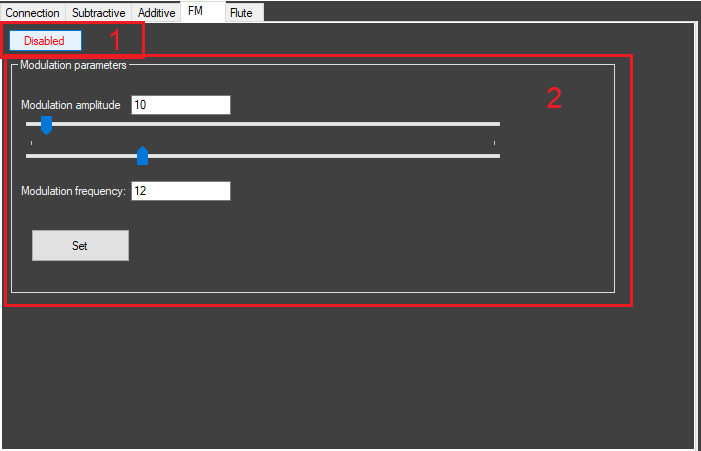
\includegraphics[width=12cm]{grafiki/fm_interface}
	\captionsetup{justification=centering}
	\caption{Interfejs użytkownika dla modulacji częstotliwości.}
	\label{rys:fm_interface}
\end{figure}
Na rysunku \ref{rys:fm_interface} zaznaczono dwie sekcje wykonanego interfejsu syntezy FM. W pierwszej z nich znajduje się przycisk, który służy do aktywacji tej metody syntezy dźwięku. Po naciśnięciu klawisza, DSP otrzymuje komunikat, po którym przechodzi w tryb syntezy FM.

W drugiej sekcji znajdują się suwaki pozwalające na wybór amplitudy oraz częstotliwości sygnału modulującego. Zmian tych wielkości można dokonywać na dwa sposoby:
\begin{itemize}
	\item z wykorzystaniem suwaków. W tym wypadku wartość ustawiona za pomocą suwaka zostanie automatycznie wpisana do pola tekstowego skojarzonego z tym regulatorem.
	\item Poprzez precyzyjne wpisanie wartości do pola tekstowego obok suwaka. W tej sytuacji regulator automatycznie się przesunie na pozycję odpowiadającą wpisanej wartości.
\end{itemize}
Wprowadzone zmiany parametrów należy zatwierdzić klawiszem "Set". Po jego naciśnięciu, odpowiednie komunikaty zostają przesłane do DSP.
